\setchapterabstract{First lecture of the precourse, it briefly covers elementary and conditional probability.}
\chapter{Elementary Probability I}
\vspace{-1.5cm}

{\chaptoc\noindent\begin{minipage}[inner sep=0,outer sep=0]{0.9\linewidth}\section{Elementary Probability}\end{minipage}}

        \subsubsection{Permutation}

        \Definition{
        any alignment in $n$ places
                    \begin{equation}
                        P_n = n!
                    \end{equation}
        }{Permutation}

        \subsubsection{Disposition}

        \Definition{
        Any alignment in $k$ places
        \begin{enumerate}
                        \item \textbf{Simple}:
                            \begin{equation}
                                D_{n,k} = n \cdot (n-1) \cdot \cdots \cdot (n-k-1) = \frac{n!}{(n-k)!}
                            \end{equation}
                        \item \textbf{With repetition}:
                            \begin{equation}
                                D_{n,k}^* = n \cdot n \cdot \cdots \cdot n = n^k 
                            \end{equation}
                    \end{enumerate}
        }{Disposition}

        \subsubsection{Combination}

        \Definition{
        any alignment of $k$ objects from $n$
                    \begin{equation}
                        C_{n,k} = \frac{n!}{k!(n-k)!} = \binom{n}{k}
                    \end{equation}
        }{Combination}

\section{Conditional Probability}

    In the probability space \( ( \Omega, A, \mathbb{P} ) \), conditional probability can be written as

    \begin{equation}
        \mathbb{P} (E|F) = \frac{\mathbb{P} (E \cap F)}{\mathbb{P} (F)}
    \end{equation}

    \noindent
    with \(\mathbb{P} (F) > 0\)

        \subsubsection{Conditional Probability as Intersection of Events}

            \begin{equation}
            \begin{split}
                \mathbb{P} (E \cap F) = & \mathbb{P} (F) \cdot \mathbb{P} (E | F) \\
                \mathbb{P} (E_1 \cap E_2 \cap \cdots \cap E_n ) = & \mathbb{P} (E_1) \cdot \mathbb{P} (E_2 | E_1) \cdot \mathbb{P} (E_3 | E_2 \cap E_1) \cdots \mathbb{P} (E_n | E_1 \cap E_2 \cap \cdots \cap E_{n-1})
            \end{split}
            \end{equation}

        \subsubsection{Law of Total Probability}

            Given \(E_1, \ E_2, \ \cdots \ E_n\) partitions of \(\Omega\) and the conditions

            \begin{enumerate}
                \item \(E_i \cap E_j = \emptyset \forall i \neq j\)
                \item \(E_1 \cup E_2 \cup \cdots \cup E_n = \Omega\)
            \end{enumerate}

            \noindent
            We can state that:

            \begin{equation}
                \mathbb{P} (F) = \sum^{n}_{i=1} \mathbb{P} (F|Ei) \mathbb{P} (E_i)
            \end{equation}

        \subsubsection{Bayes Formula}

            Given 

            \begin{equation}
                \mathbb{P} (E_n | F) = \frac{\mathbb{P} (F| E_n) \mathbb{P} (E_n)}{\sum^{n}_{i=1} \mathbb{P} (F|Ei) \mathbb{P} (E_i)} \rightarrow \mathbb{P} (A|P) \frac{\mathbb{P} (B|A) \mathbb{P} (A)}{\mathbb{P} (B)}
            \end{equation}

\section{Independent Events}

        \subsubsection{Stochastic Independence}

            \Definition{
            Given the probability space \( ( \Omega, A, \mathbb{P} ) \), two events \(E, F \in A\) are said to be \textbf{stocastically independent} if \(\mathbb{P} (E) \cap \mathbb{P} (F) = \mathbb{P} (E) \cdot \mathbb{P} (F)\)
            \begin{equation}
                \mathbb{P} (E|F) = \mathbb{P} (E) \iff \mathbb{P} (F|E) = \mathbb{P} (F)
            \end{equation}
            }{Stochastic Independence}
            

        \subsubsection{Conditional Stochastic Independence}

            \Definition{
            Given the probability space \( ( \Omega, A, \mathbb{P} ) \) and the events \(A, B, F \), \textbf{Conditional Stochastic Independence} can be characterised as:
            \begin{equation}
                \mathbb{P} (A \cap B | F) = \mathbb{P} (A|F) \cdot \mathbb{P} (B|F)
            \end{equation}
            }{Conditional Stochastic Independence}

            \Warning{
            Stochastic Independence \textbf{does not imply} Conditional Stochastic Independence, and vice versa.
            }
            

\section{Random Variables}

        Given the sample space of tossing a dice \(\Omega = \{1,2,3,4,5,6\} \), we can define:

            \[X: \Omega \rightarrow \mathbb{R} \]

        \Remark{
        In the equation above:
                \begin{itemize}
                    \item if \(\Omega\) is finite \(\rightarrow\) it is a random variable
                    \item if \(\Omega\) is discrete \(\rightarrow\) it is \textbf{not} a random variable 
                \end{itemize}
        }

        \noindent
        Properties to be considered a random variable:

            \begin{itemize}
                \item \(\forall t \in \mathbb{R}\)

                    \( \{ \omega \in \Omega : X (\omega) \leq t \} = E_t \in A \)

                    With \(X\) being \textbf{Borel measurable}

                \item 

                    \( \mathbb{P} (E_t) = \mathbb{P} (\omega \in \Omega : X (\omega) \leq t ) = \mathbb{P} (X (\omega) \leq t) = \mathbb{P} (X \leq t)  0 F_x (t)  \)
 
                \item \(F_x : \mathbb{R} \rightarrow \mathbb{R}\), with \(F_x(t)\) being the distribution function of the variable.

                    \( \lim _{t \to - \infty} F(t) = 0 \)    

                    \( \lim _{t\to\infty} F(t) = 1\)

                    \begin{itemize}
                        \item If \(X\) is discrete, the graph will possess the following properties:
                            \begin{enumerate}
                                \item Stepwise
                                \item Non-decreasing 
                                \item \(F_x\) continuous from the right
                            \end{enumerate}
                        \item If \(X\) is \textcolor{dblue}{absolutely} continuous
                            \begin{enumerate}
                                \item \(F\) is continuous
                            \end{enumerate}
                    \end{itemize}
            \end{itemize}

            \begin{figure}[h]
                \centering
                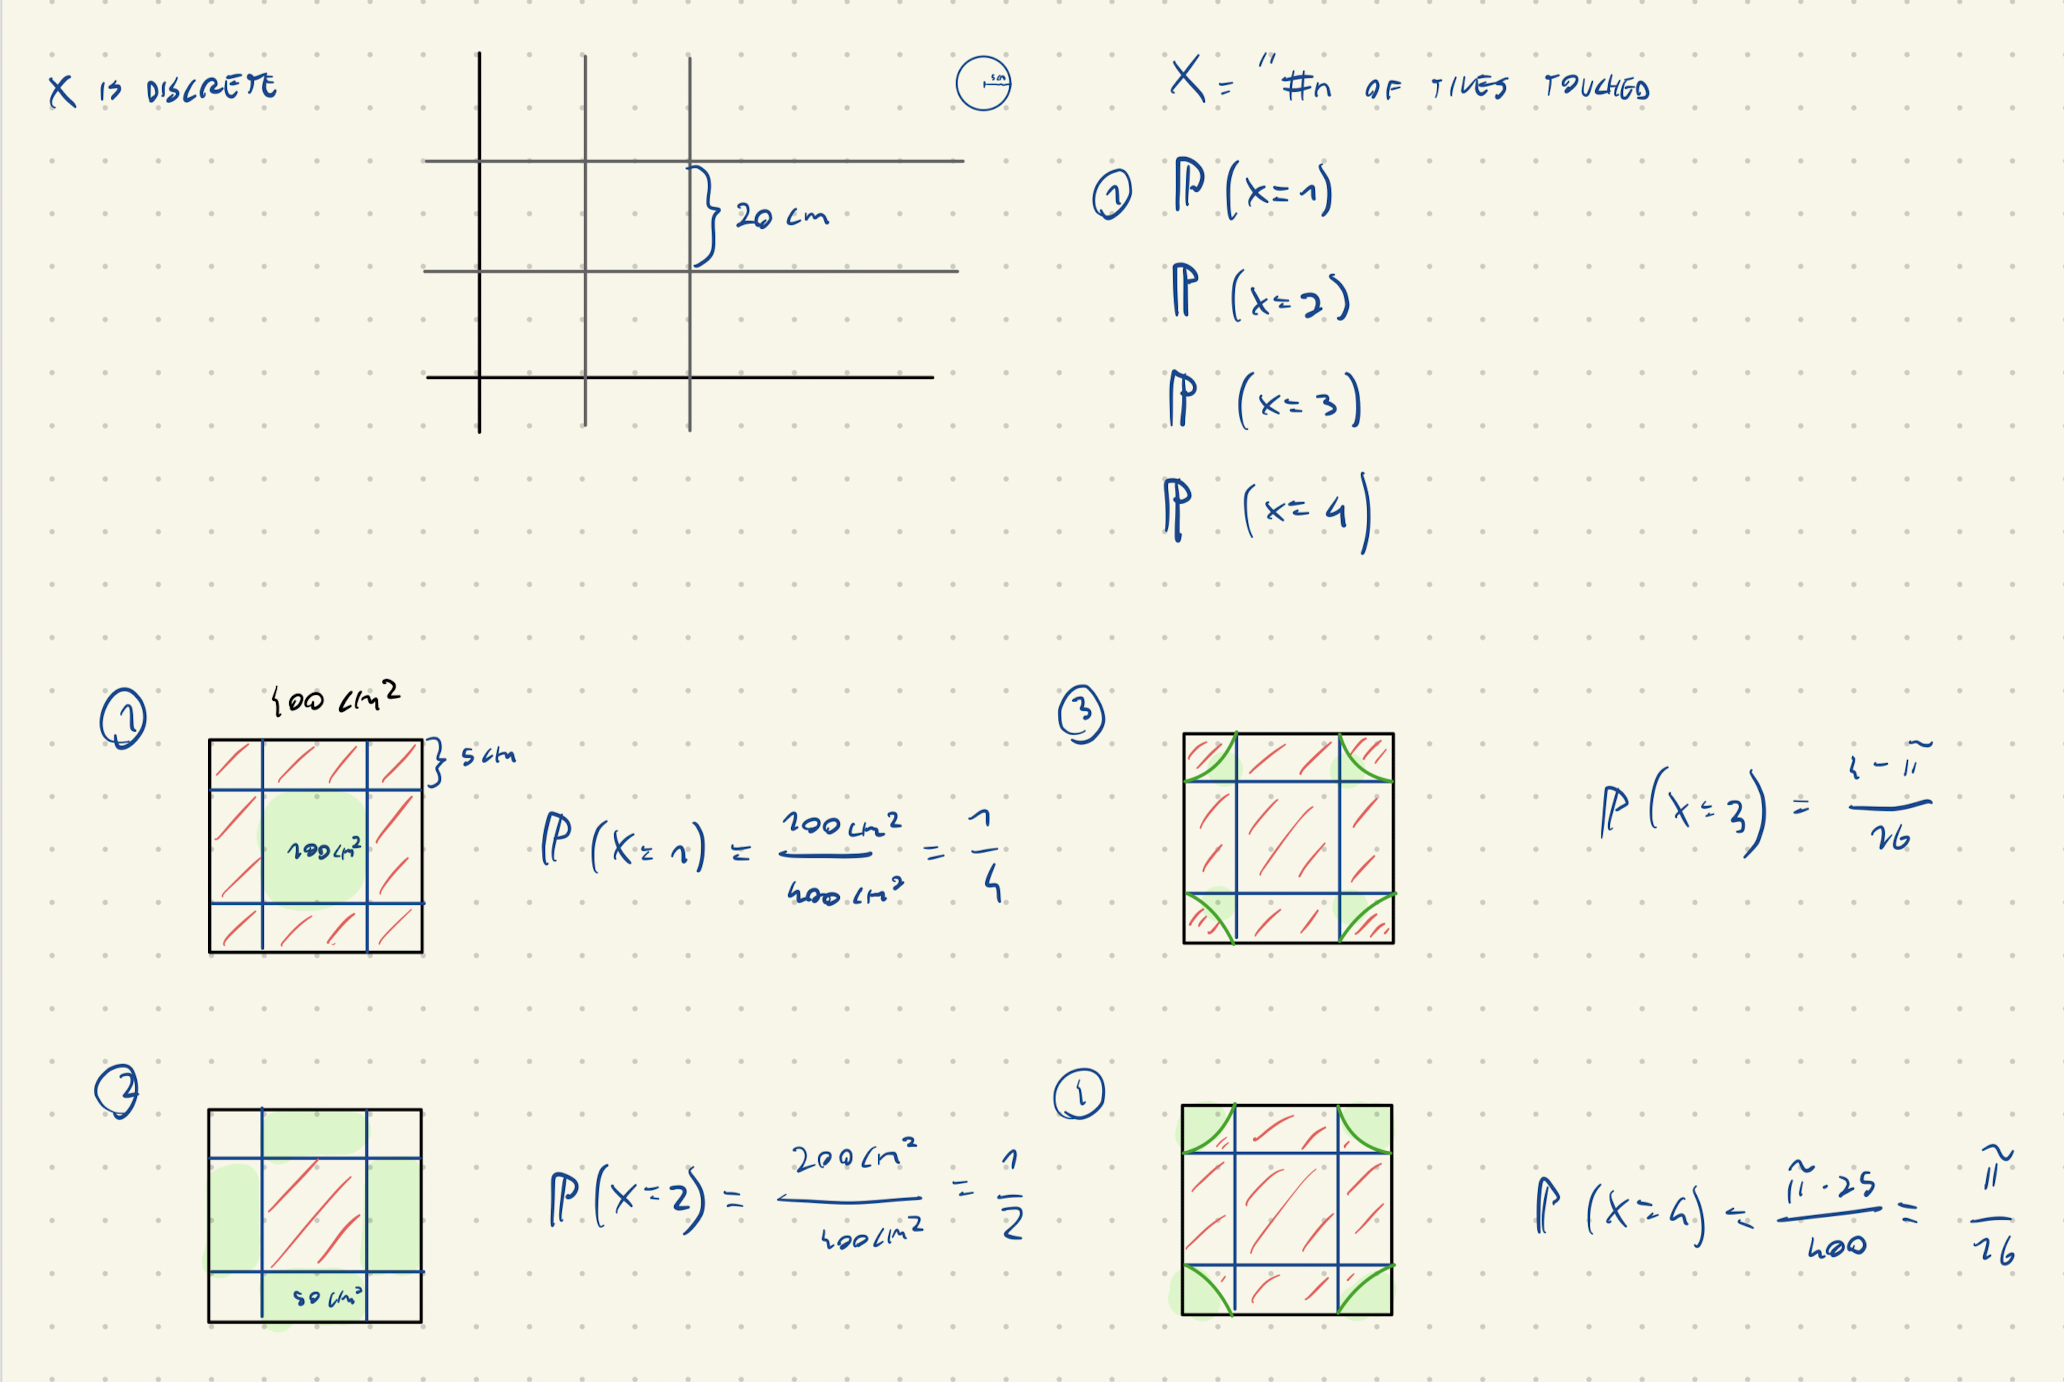
\includegraphics[width=0.90\linewidth]{X_visual_discrete.png}
                \caption{Visual representation of an example where \(X\) is a \textbf{discrete} random variable}
                \label{fig:X_visual_discrete}
            \end{figure}

            \begin{figure}[h]
                \centering
                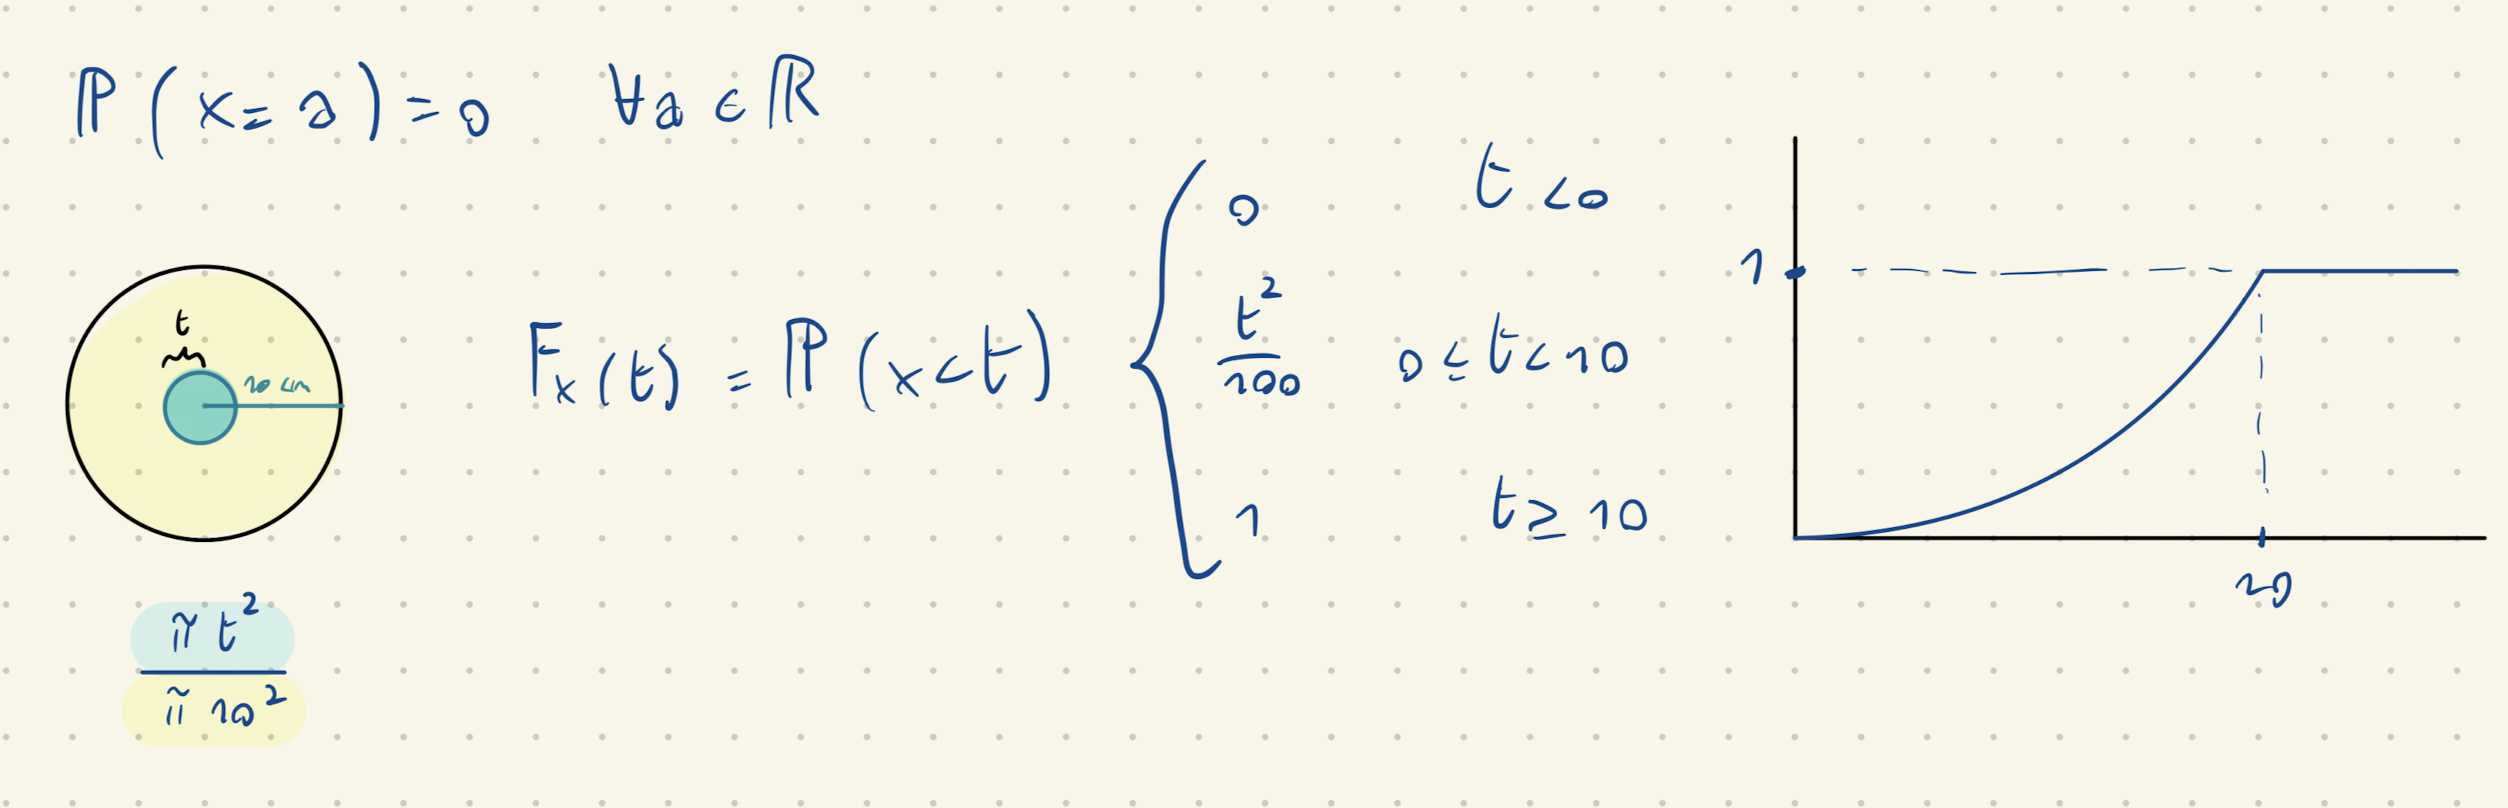
\includegraphics[width=0.90\linewidth]{X_visual_absolutely_continuous.png}
                \caption{Visual representation of an example where \(X\) is an \textbf{absolutely continuous} random variable}
                \label{fig:X_visual_absolutely_continuous}
            \end{figure}

\newpage
\section{Probability Density Function | \(f(x)\)}

        \begin{equation}
        \begin{split}
            \probP (a < X \leq b) = \probP (X \leq b) - \probP (X \leq a) = & \overbrace{F_x (b)}^{CDF} - F_x (a) \\
            = & \int_{a}^{b} \underbrace{f(x)}_{PDF} dx
        \end{split}     
        \end{equation}
            
        \Note{
        Relationship between Cumulative Distribution Function and Probability Density Function:
        \[f_x (x) = \frac{d}{dx} F_x (X) \iff F_x (t) = \int_{-\infty}^{t} f_{x} (x) dx \]
        }

\newpage
        \subsection{Properties of the Probability Density Function}

            \begin{enumerate}
                \item \textbf{Non Negativity}: the density is never negative

                    \begin{equation}
                        f_x (x) \geq 0 \ \forall x \in \mathbb{R}
                    \end{equation}
                    
                \item \textbf{Normalisation}: the area below the curve of the density function is always equal to 1

                    \begin{equation}
                        \int_{-\infty}^{\infty} f_x (x) dx = 1
                    \end{equation}
                    
            \end{enumerate}

        \Example{
        \begin{equation}\label{example-pdf-1}
                f_x(x) = \begin{cases} cx^2 & \mbox{if } -1 < x \leq 2 \\ 0 & \mbox{a.e.} \end{cases}
            \end{equation}
            \[1 = \int_{-\infty}^{\infty} f_x (x) dx =  \underbrace{\int_{-\infty}^{-1} f_x (x) dx}_{=0} + \int_{-1}^{2} f_x (x) dx + \underbrace{ \int_{2}^{\infty} f_x (x) dx}_{=0} = \int_{-1}^{2} f_x (x) dx =  \]
            \[\int_{-1}^{2} cx^2 dx =\left[c \frac{x^3}{3}\right]_{-1}^{2} = \frac{c}{3} (8+1) = 3c \rightarrow 3c = 1 \rightarrow c = \frac{1}{3} \]
            Given the function \(c \cdot x^2\), the constant \(c\) that allows the function to respect the properties of a \textit{probability density function} is \(c = \frac{1}{3}\).
            The final form of function \ref{example-pdf-1} is hence:
            \[
                f_x(x) = \begin{cases} \frac{1}{3} x^2 & \mbox{if } -1 < x \leq 2 \\ 0 & \mbox{a.e.} \end{cases}
            \]
        }

        \Example{
        Imagine there is a traffic light, where the \textcolor{ForestGreen}{green light} lasts for 20' and the \textcolor{BrickRed}{red light} lasts for 40'. Define \(X\) as the waiting time. (Note: X is neither discrete nor continuous).
            \begin{equation}\label{example-pdf-2}
                F_x(t) = \begin{cases} 0 & \mbox{if } t<0 \\ \clubsuit & \mbox{if } 0 \leq t < 40 \\ 1 & \mbox{if } t \geq 40 \end{cases}
            \end{equation}
            \[
            \clubsuit = \probP (x \leq t) = \probP (x \leq t | \textcolor{BrickRed}{R}) \cdot \probP (\textcolor{BrickRed}{R}) + \probP (x \leq t | \textcolor{ForestGreen}{G}) \cdot \probP (\textcolor{ForestGreen}{G}) = 
            \]
            \[
            \frac{t}{40} \cdot \overbrace{\frac{40}{20+40}}^{prob. \ light=\textcolor{BrickRed}{R}} + 1 \cdot \overbrace{\frac{20}{20+40}}^{prob. \ light = \textcolor{ForestGreen}{G}} =  
            \]
            \[
            \clubsuit = \frac{1}{3} \cdot \frac{t+20}{60}
            \]
        }

\newpage
\section{Expected Value}

    The expected value of a probability function can be described as:

        \begin{equation}
            E(x)= \int_{0}^{+\infty} (1-F_x(t)) dt - \int_{-\infty}^{0} F_{x}(t) dt \begin{cases}
                \sum x_i p_x (I) & \mbox{if $X$ is discrete} \\ \int_{-\infty}^{+\infty} x f_x(x) dx & \mbox{if $X$ is continuous} \end{cases}
        \end{equation}

    \Example{
        When X = \textit{number of tiles}:
        \[E(x) = 1 \cdot \frac{1}{4} + 2 \cdot \frac{1}{2} + 3 \cdot \frac{4-\pi}{16} + 4 \cdot \frac{\pi}{16} = 2+ \frac{\pi}{16} \]
    }

    \Example{
        When X = \textit{distance from centre}:
        \[E(x) = \int_{-\infty}^{+\infty} x f_x(x) dx \Rightarrow E(x) = \int_{0}^{10} x \frac{2x}{100} dx = \left[ \frac{2}{100} \frac{x^3}{e} \right]_0^{10} \]
    }

    \Example{
        When X = \textit{waiting time at the traffic light}:
        \[E(x) = \int_{-\infty}^{+\infty} x f_x(x) dx = \underbrace{\int_{-\infty}^{0} F_x(t)dt}_{=0} + \int_{0}^{+\infty} 1-F_x(t)dt\]
        \[ \int_{0}^{40} 1- \left( \frac{20+t}{60} \right) = \left[ \frac{1}{60} \left( 40t - \frac{t^2}{2} \right) \right]^{40}_0 = 13.\Bar{3} \]
    }

    \subsection{Properties of the Expected Value}

        Given \(Y=g(X)\), it can be shown that

        \begin{equation}\label{Properties-of-the-Expected value}
            E(Y) = E(g(X))
        \end{equation}

        which can be evaluated without knowing the distribution of $Y$ but only the function \(g(X)\).

        \Example{
        Say we want to calculate the expected value of a function \(g(X) = x^2\).
        \begin{itemize}
            \item \textbf{if \(x\) is discrete}
                \[\sum x_i^2 p_x (x_i)\]
            \item \textbf{if \(x\) is absolutely continuous}
                \[\int_{-\infty}^{+\infty} x^2 f(x) dx \]
        \end{itemize}
        }

\section{Variance}

    \Definition{
    The variance \(Var\) of a random variable \(X\) can be defined as:
        \begin{equation}
            Var(X) = E \left[ ( X-\overbrace{E(X)}^{=m} )^2 \right] = E \left[ (\underbrace{X}_{r.v.}-\overbrace{m}^{\in \mathbb{R}})^2 \right]
        \end{equation}
    Alternatively, one may employ the following shortcut:
        \[ E \left[ (x-m)^2 \right] = E(X^2) + \underbrace{E(m^2)}_{m^2} -2mE(X) = E(X^2) +m^2 -2m^2 = E(X^2)-m^2 \]
    }{Variance}
    
    \subsection{Chebyshev Inequality}

        \Definition{
        Chebyshev inequality  provides an upper bound on the probability of deviation of a random variable (with finite variance) from its mean.
        \begin{equation}
             \mathbb{P}(|X-E(x) |\geq \eta )\leq {\frac {Var(X)}{\eta^{2}}}
        \end{equation}
        Moreover, expressing the \textit{standard deviation} of \(x\) as \(\sqrt{Var(X)} = s\), we can rewrite the equation as follows:
            \[ \mathbb{P}(|X-E(x) |\geq k )\leq {\frac {s^2}{k^{2}}} \]
        }{Chebyshev Inequality}

        \Remark{
        When dealing with variance, we ought to keep in mind that
        \[Var(aX+b) = a^2 Var(X) \]
        }

        \subsubsection{Discrete Case}

            \Example{
            Suppose we have a random variable \(X\) distributed such that
            \begin{center}
                \begin{tabular}{|c|c|c|}
                    1 & 2 & 3 \\
                    0.2 & 0.5 & 0.3
                \end{tabular}
            \end{center}
            In order to find the variance \(Var(X)\), let's first find the expected value of the random variable \(E(X)\) and of the random variable squared \(E(X^2)\).
            \[E(X) = 1 \cdot 0.2 + 2 \cdot 0.5 + 3 \cdot 0.3 = 1.7 \]
            \[E(X^2) = 1^2 \cdot 0.2 + 2^2 \cdot 0.5 + 3^2 \cdot 0.3 = 4.9 \]
            \[Var(X) = E(X^2) - E(X)^2 = 2.01 \]
            }
        
        \subsubsection{Continuous Case}

            \Example{
            Suppose we have a random variable \(X\) distributed such that
            \begin{equation}
                f_x(x) \begin{cases}
                    \frac{1}{2 \sqrt{x}} & 0 < x < 1 \\ 0 & \mbox{a.e.} \end{cases}
            \end{equation}
            The first step is to find the cumulative distribution function \(F_X(t)\)
            \[F_X(t) = \int_{-\infty}^{+\infty} \frac{1}{2\sqrt{x}} dx \rightarrow F_X(t) \begin{cases}
                0 & t < 0 \\
                \sqrt{t} & 0 \leq t < 1 \\
                1 & t \geq 1
            \end{cases} \]
            We now move on to \(E(X)\) and \(E(X^2)\)
            \[E(X) = \int_{-\infty}^{+\infty} x \cdot  \frac{1}{2\sqrt{x}} dx\]
            \[E(X^2) = \int_{-\infty}^{+\infty} x^2 \cdot \frac{1}{2\sqrt{x}} dx \]
            }

FINE